\section{如何申请数据中心税收优惠}

\subsection{得克萨斯州}

申请人必须向得克萨斯州审计长办公室提交 AP-233 或 AP-236 表格，登记为符合条件的数据中心或大型数据中心项目，并取得唯一登记编号。随后，申请人须向销售方提供免税证书（01-929 表格），以申请免税待遇。

申请时必须附上资本投入计划、就业创造计划，以及场地平面图或建筑示意图。

\begin{figure}[htbp]
\centering
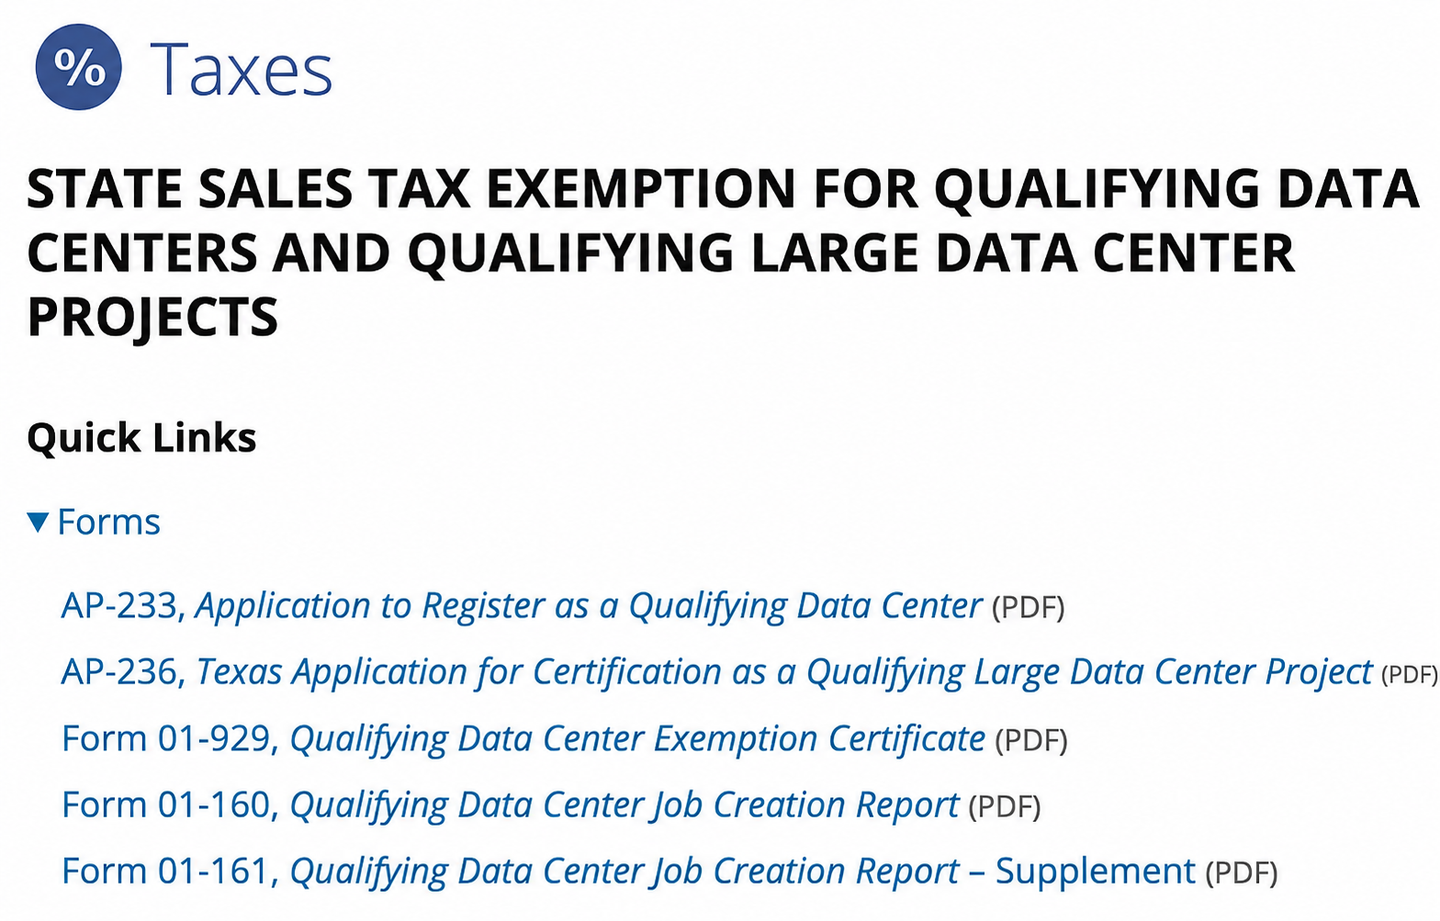
\includegraphics[width=0.48\linewidth,height=0.34\textheight,keepaspectratio]{assets/figure-5.png}\hfill
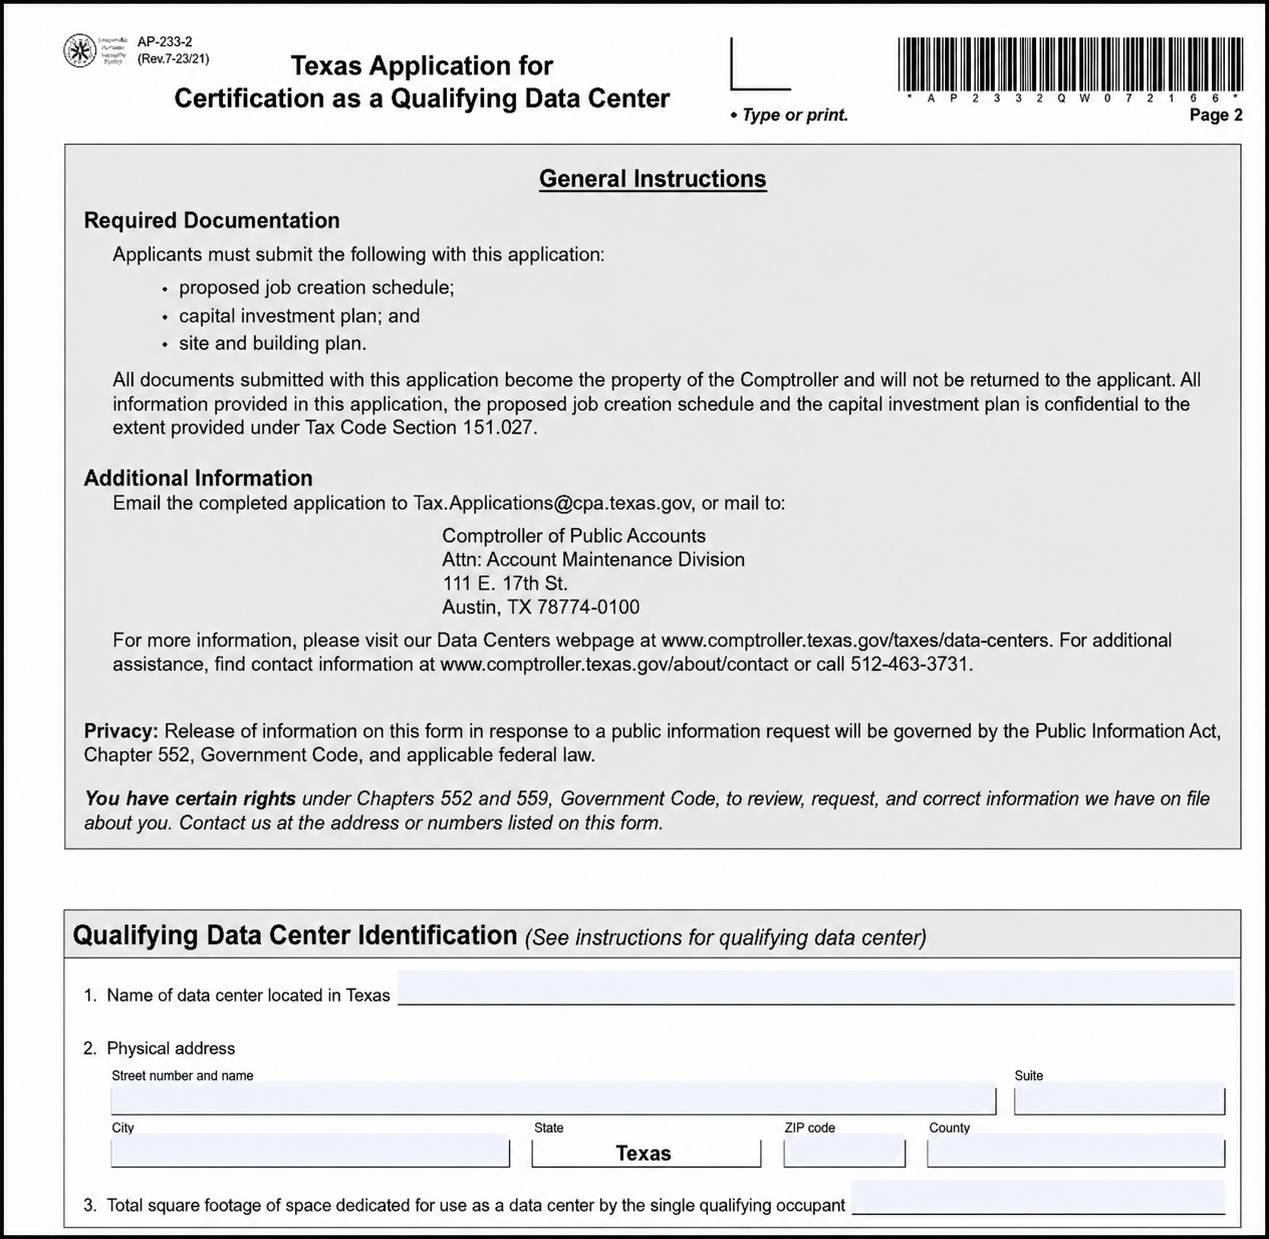
\includegraphics[width=0.48\linewidth,height=0.34\textheight,keepaspectratio]{assets/figure-6.png}
\caption{得克萨斯州合资格数据中心申请表下载页面（原文图2、图3；保留英文截图）}
\end{figure}

申请表下载：

\url{https://comptroller.texas.gov/taxes/data-centers}

\FloatBarrier
\subsection{弗吉尼亚州}

申请 DCRSUT 豁免时，符合条件的数据中心必须与弗吉尼亚州经济发展合作署（VEDP）协商并签署谅解备忘录（MOU）。VEDP 将备忘录提交州税务部门审查；获批后，税务部门直接向数据中心签发免税证书。

托管数据中心的租户须另行与数据中心签署参与证书及协议。VEDP 与州税务部门审查相关参与证书及协议后，税务部门直接向租户签发单独的免税证书。

谅解备忘录下载：

\url{https://www.vedp.org/incentive/data-center-retail-sales-use-tax-exemption}

\subsection{佐治亚州}

数据中心所有者或高科技数据中心客户，可通过佐治亚州税务中心（GTC）提交免税证书申请。在相应数据中心所有者取得免税证书之前，税务部门不会向客户签发证书。

申请过程中，数据中心可能需要提供申请人在佐治亚州的所得税申报和缴纳记录、申请人对该州不动产拥有的产权或权益价值、足以证明其可能满足高科技数据中心最低投资门槛的文件，以及其他支持材料。高科技数据中心客户还可能需要提交数据中心服务合同副本等文件。

申请说明：

\url{https://dor.georgia.gov/how-apply-high-technology-data-center-exemption}

\FloatBarrier
